\documentclass[12pt]{beamer}
\usepackage[utf8]{inputenc}
\usepackage[spanish]{babel}
%\usepackage[dvips]{epsfig}
\usepackage{graphics}
\usepackage{url}
\usepackage{ulem}
\usepackage{beamerthemesplit}
\usepackage{color}
\usepackage{hyperref}
\usepackage{wrapfig}
\usetheme{CambridgeUS}

\title{Innovar o Morir}
\subtitle{Taller de Gestión de Proyectos Informáticos}
\author[R. Fernández]{Rodrigo Fernández \\ \small{\texttt{rfernand@inf.utfsm.cl}}}
\institute[]{Universidad Técnica Federico Santa María}
\titlegraphic{
\includegraphics[height=1cm]{img/logos}}
\date{\today}

\begin{document}
    \frame{\titlepage}
    \frame{\tableofcontents}
	\section{¿Qué es innovar?}
    \begin{frame}[fragile]
\frametitle{Innovación}
\begin{table}
\begin{tabular}{p{7cm}p{3cm}}
\small
\begin{verbatim}
«La innovación por la innovación no sirve para nada.
Innovar es crear productos que hagan la vida más fácil.»
\end{verbatim}&\\
\normalsize
\begin{itemize}
    \item Creación o modificación de un producto y su introducción en un
    mercado.
    \item Renovar, introducir una novedad.
\end{itemize}
&
\vspace{1cm}
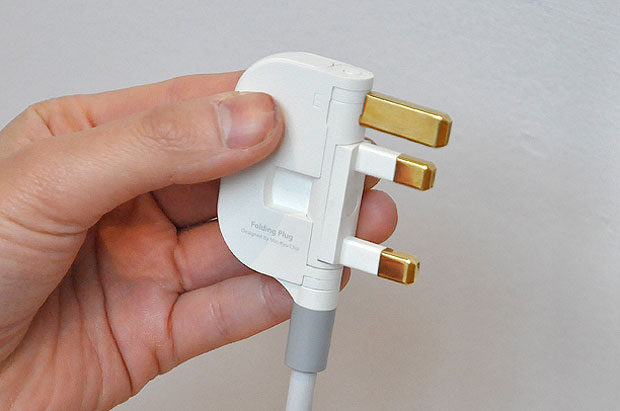
\includegraphics[width=4cm]{img/enchufe.jpg}\\
\end{tabular}
\end{table}
\end{frame}


	\section{Estrategias para no morir}
    \frame
{
\frametitle{Venta de la licencia de su tecnología más avanzada}
\begin{table}
\begin{tabular}{p{7cm}p{3cm}}
\begin{itemize}
    \item Vender ideas en cuanto son comercializables.
    \item Imponerse a propósito más presión sobre sí mismo.
\end{itemize}
&
\vspace{1.5cm}

\includegraphics[width=4cm]{img/innovar.jpg}\\
\end{tabular}
\end{table}
}

\frame
{
\frametitle{Canibalice sus productos más rentables}
\begin{table}
\begin{tabular}{p{7cm}p{3cm}}
\begin{itemize}
    \item Lanzar nuevos productos sin importar que compitan con los viejos
    productos de la empresa.
\end{itemize}
&
\vspace{1.5cm}
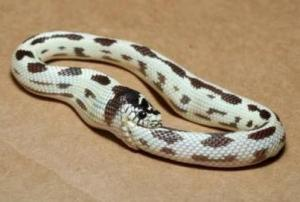
\includegraphics[width=4cm]{img/ouroboros.jpg}\\
\end{tabular}
\end{table}
}
\frame
{
\frametitle{Venda/divida nuevas unidades}
\begin{table}
\begin{tabular}{p{7cm}p{3cm}}
\begin{itemize}
    \item Cultura organizacional no permite diferentes enfoques.
    \item Equipos paralelos de trabajo.
\end{itemize}
&
\vspace{1.5cm}
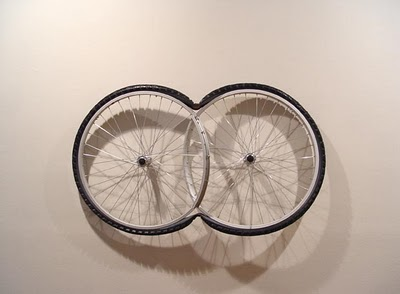
\includegraphics[width=4cm]{img/mitosis.jpg}\\
\end{tabular}
\end{table}
}
\frame
{
\frametitle{Liquide los viejos éxitos para forzar la dependencia de los nuevos}
\begin{table}
\begin{tabular}{p{7cm}p{3cm}}
\begin{itemize}
    \item \textit{Deshacerse} de uno o más productos muy rentables, mientras
    todavía sean rentables.
    \item Obliga a depender de las líneas más nuevas del negocio.
\end{itemize}
&
\vspace{1.5cm}

\includegraphics[width=4cm]{img/getting_older.jpg}\\
\end{tabular}
\end{table}
}
\frame
{
\frametitle{Financie la audacia}
\begin{table}
\begin{tabular}{p{7cm}p{3cm}}
\begin{itemize}
    \item Financiar a las \textit{mentes brillantes} de la propia empresa.
    \item Evita que éstas abandonen la empresa, o caigan sofocados bajo
    prejuicios.
    \item Ser un \textit{Capitalista de Riesgo}.
\end{itemize}
&
\vspace{1.5cm}

\includegraphics[width=4cm]{img/creativegenius.jpg}\\
\end{tabular}
\end{table}
}
\frame
{
\frametitle{Vender cuota sustancial de los productos o servicios al mercado
exterior}
\begin{table}
\begin{tabular}{p{7cm}p{3cm}}
\begin{itemize}
    \item Demostrar aptitud para competir.
    \item Cada unidad de la empresa debe estar involucrado.
    \item Competir contra los mejores.
\end{itemize}
&
\vspace{1.5cm}

\includegraphics[width=4cm]{img/openbusiness.jpg}\\
\end{tabular}
\end{table}
}
\frame
{
\frametitle{Forzar la competencia entre las funciones internas con las
externas.}
\begin{table}
\begin{tabular}{p{7cm}p{3cm}}
\begin{itemize}
    \item Estimular que las unidades cercanas al mercado compren los mejores
    productos y servicios, incluyendo a los de la competencia.
\end{itemize}
&
\vspace{1.5cm}

\includegraphics[width=4cm]{img/competition.jpg}\\
\end{tabular}
\end{table}
}
\frame
{
\frametitle{Subcontrate absolutamente todo}
\begin{table}
\begin{tabular}{p{7cm}p{3cm}}
\begin{itemize}
    \item Subcontratación como forma de vida.
    \item Red de subcontratistas.
    \item La innovación es lo importante.
\end{itemize}
&
\vspace{1.5cm}
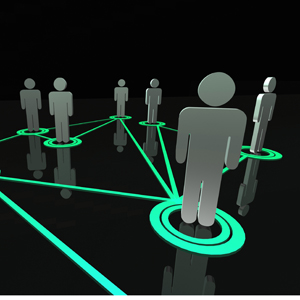
\includegraphics[width=4cm]{img/subcontract.jpg}\\
\end{tabular}
\end{table}
}
\frame
{
\frametitle{Crear numerosas joint-ventures y alianzas}
\begin{table}
\begin{tabular}{p{7cm}p{3cm}}
\begin{itemize}
    \item Trabaje con todo el mundo, de cualquier parte, durante un periodo
    corto o largo.
    \item Especialmente con empresas nuevas y del exterior.
\end{itemize}
&
\vspace{1.5cm}

\includegraphics[width=4cm]{img/joint-venture.jpg}\\
\end{tabular}
\end{table}
}

    \section{Conclusiones}
    %De acuerdo a la introducci\'on que se hizo, entregar afirmaciones
%  basadas en los experimientos y sus resultados.

A primera vista, los resultados obtenidos en la presente implementación, superan en gran medida a los óptimos encontrados
en todos estos años, donde distintas personas, han utilizado, variadas técnicas para poder resolver el \emph{Car Sequencing Problem}
de la mejor manera, considerando así, que se pudieron haber utilizado técnicas completas, que si bien es cierto, pueden demorar mucho,
van a encontrar el \emph{óptimo global} de un determinado problema, lo cual se diferencia notoriamente con las técnicas incompletas,
como es el caso de ka presente implementación, donde sólo se puede encontrar un \emph{óptimo local}.

Al mirar el gráfico podemos darnos cuenta, de que la distribución de la cantidad de restricciones violadas, poseen un comportamiento
bastante similar, guardando las proporciones de la cantidad de violaciones, lo que nos hace deducir, de que sólo nos falta un poco
más de control y sintonización de los parámetros utilizados, para acercarnos aún más a soluciones más óptimas.

Siguiendo con el análisis de los experimentos, podemos darnos cuenta de que si bien es cierto, las soluciones violan una cantidad
considerable de restricciones, estamos sacrificando una buena solución, por un corto tiempo de ejecución, el cual en algunos casos,
sólo llega a durar 1 minuto, lo que comparado con el tiempo de alguna técnica completa, que puede durar días, nos beneficia de cierta manera.

Con respecto a la representación del problema, existen ciertos pros y contras.
Primero que todo la representación que se utilizó en la presente implementación,
consiste en una del tipo no-binaría, por lo que no es tan fácil utilizar los típicos movimientos de las representaciones binarias,
como lo son el \emph{bit-flip} y el \emph{cruzamiento en un punto}, ya que estaríamos violando las restricciones duras del problema,
por lo cual en la presente implementación, por ejemplo, no se utilizó un operador de cruzamiento y sólo se deposito la confianza,
en la mutación con \emph{Simulated Annealing} que se encargó tanto de explorar como de explotar.

Según lo anteriormente dicho, el no poseer un operador de cruzamiento, puede haber perjudicado la explotación del presente algoritmo
evolutivo, y por ende, entorpecido la búsqueda de un óptimo local. Aunque los resultados no fueron del todo malos, por lo que el simulated annealing
hizo su trabajo explorando y explotando, pero no de la forma más apropiada.

Otro punto importante en la presente implementación, es la forma en la cual se genera la población inicial.
Como ya hemos mencionado anteriormente, lo favorable del método utilizado es que se generan soluciones factibles,
es decir, que cumplen las restricciones duras, pero por otro lado, éstas se generan de forma aleatoria, lo cual indica,
que quizás utilizando alguna técnica de construcción de individuos más apropiada, como Greedy o GRASP, la calidad de la
población inicial aumentaría, lo cual sería interesante como trabajo futuro.


Con respecto a la mutación con simulated annealing, cabe señalar que existen algunos aspectos que pueden ser mejorados,
como por ejemplo un control de la temperatura, pues en la presente implementación, la temperatura disminuye cada 3 iteraciones,
lo que si tomamos en cuenta un control más riguroso, como comparar la calidad de las soluciones generadas, podríamos
realizar los cambios en la temperatura, a medida que el algoritmo se comporta de una forma más apropiada.


Finalmente, es posible mejorar la presente implementación de un algoritmo evolutivo aumentando la exploración,
que en éste caso significa poder mejorar lo que es la mutación, ya que dentro del simulated annealing, el movimiento
no es muy apropiado, y quizás el sólo hecho de mejorar el movimiento de la mutación simulated annealing, puede
traer un mejor desempeño en nuestro algoritmo. Otra forma podría ser cambiar el método de la ruleta, pues si bien es cierto,
le entrega una mayor probabilidad para escoger los mejores individuos, no nos prohibe elegir malos individuos, lo que
perjudica a nuestra siguiente población, y por ende a la solución del problema.


% OLD

%Conclusiones revelantes del estudio realizado.

%En el presente informe se ha dado un estado del arte de un problema muy popular
%en el área de la inteligencia artificial, el \emph{Car Sequencing Problem}, siendo éste
%una variación de otro problema connotado llamado \emph{Job Shop Scheduling}.
%Es tanto la importancia del presente problema, que la \emph{French Society of Operations
%Research and Decision-Making Aid} ha decidido ya hace varios años, comenzar lo que se denomina
%\emph{The ROADEF challenge} cada dos años, teniendo como objetivo central,  permitir a las personas
%que se desarrollan en el área de la industria el presenciar todos los avances y evoluciones
%en el ámbito de la Investigación de Operaciones y Análisis de Decisiones, pero no sólo eso
%sino el poder enfrentar directamente problemas decisionales complejos, que ocurren en la industria.
%Siguiendo la idea anterior, lo importante de éste \emph{Challenge} es que en el 2005, se consideró
%como tema principal el \emph{Car Sequencing Problem} debido a la propuesta que realizó RENAULT,
%por lo cual uno podrá imaginar la cantidad de avances que se produjeron, pues cada participante
%abordaba el problema desde una metodología distinta.
%
%Por otra parte, pareciera que un problema relacionado a \emph{ordenar} un conjunto de vehículos
%para ser ensamblados y así obtener el orden más óptimo, no es una tarea difícil, pero claramente
%debido a la complejidad que otorgan las restricciones y de que es un problema de la vida real,
%presenta un grado de dificultad mayor, lo cual queda reflejado por la cantidad de publicaciones 
%e investigaciones que hay al respecto.
%
%Se dieron a conocer también, tres áreas para atacar el presente problema.
%Por un lado tenemos los métodos heurísticos que como bien sabemos, es prácticamente jugar a la ruleta
%rusa con nuestra investigación, pues la heurística solamente selecciona un objetivo de los dos provenientes
%de la definición, una buena solución o un buen tiempo de ejecución. Pero también se presenta que la heurística
%es un mecanismo confiable para decidir \emph{utilizarlo} como un apoyo, mas que utilizarlo solo.
%
%Siguiendo con los mecanismos planteados, se vieron también los  métodos exactos,
%es decir, técnicas de optimización, donde podemos encontrar la \emph{programación lineal entera},
%\emph{branch and bound} y \emph{local search}, los cuales se dedicaban netamente a construir una
%solución óptima a partir de los datos que el mismo problema nos entrega. El único problema que tienen
%éstas técnicas es que la complejidad temporal va a crecer demasiado con respecto al tamaño de nuestro
%\emph{input} del algoritmo.
%
%Dentro de toda la lectura realizada para las distintas técnicas, pude percatarme que las mejores soluciones
%siempre son variaciones de métodos o tomar dos técnicas como complementarias, por ejemplo uno de los
%mejores resultados fue la combinación de un \emph{Ant Colony Optimization} con una heurística dinámica,
%pues claramente se nos señala que el buen uso de una heurística es crucial, es decir, hay que preocuparse
%de leer los estudios que se han publicado, par ver cual es la combinación más óptima.
%
%Finalmente, es impresionante la cantidad de estudios con respecto a éste problema en particular,
%por lo que podemos darnos cuenta que muchos centros de investigación han dedicado tiempo valioso
%para la resolución óptima del \emph{Car Sequencing Problem}, pero no tanto la versión que se estudió,
%que es la propuesta por Parello~\cite{parello}, sino mas bien al desafío de la ROADEF.

\end{document}
